
%%%%%%%%%%%%%%%%%%%%%%%%%%%%%%%%%%%%%%%% IMPORTS %%%%%%%%%%%%%%%%%%%%%%%%%%%%%%%%%%%%%%%%
\documentclass[10pt,onesize,a4paper,titlepage]{article}

%%%%%%%%%%%%%%% Formatting %%%%%%%%%%%%%%%
\usepackage[english]{babel}
\usepackage[utf8]{inputenc}
\usepackage{geometry} % Margins
\usepackage{sectsty} % Custom Sections
\usepackage{paralist} % For compactitem

%%%%%%%%%%%%%%% Font %%%%%%%%%%%%%%%
%\usepackage{Archivo}
\usepackage[T1]{fontenc}
\renewcommand{\familydefault}{\sfdefault} % Set Helvetica default

%%%%%%%%%%%%%%% Graphics %%%%%%%%%%%%%%%
\usepackage{fontawesome5} % Icons
\usepackage{graphicx} % Images
\usepackage[most]{tcolorbox} % Color Box
\usepackage{xcolor} % Colors
\usepackage{tikz} % For Drawing Shapes
\tcbuselibrary{breakable}

%%%%%%%%%%%%%%% Miscelanous %%%%%%%%%%%%%%%
\usepackage{lipsum} % Lorem Ipsum
\usepackage{hyperref} % For Hyperlinks

%%%%%%%%%%%%%%% Colors %%%%%%%%%%%%%%%
%\definecolor{accent}{HTML}{9fbfc0} % Accent color
\definecolor{accent}{HTML}{585AFE} % Accent color
\definecolor{lightgrey}{HTML}{d2d2d2} % Title color
\definecolor{skillbar}{HTML}{ffffff} % Empty skill bars

%%%%%%%%%%%%%%% Section Format %%%%%%%%%%%%%%%

% Change font of \section command
\sectionfont{
	\Large
	\fontseries{m}\selectfont
	\sectionrule{0pt}{0pt}{-8pt}{1pt}
}

\subsectionfont{
	\large
	\fontseries{m}\selectfont
	\sectionrule{0pt}{0pt}{-8pt}{1pt}
}

%%%%%%%%%%%%%%% Margins and Headers %%%%%%%%%%%%%%%
\geometry{
	a4paper,
	left=7mm,
	right=7mm,
	bottom=10mm,
	top=10mm
}

\pagestyle{empty} % Empty Headers



%%%%%%%%%%%%%%%%%%%%%%%%%%%%%%%%%%%%%%%% MACROS %%%%%%%%%%%%%%%%%%%%%%%%%%%%%%%%%%%%%%%%

%%%%%%%%%%%%%%% Link With an Icon %%%%%%%%%%%%%%%
\newcommand{\link}[1]{
	\href{#1}{\faIcon{link}}
}

%%%%%%%%%%%%%%% Name Template %%%%%%%%%%%%%%%
\newcommand{\name}[2]{
	% Name
	\Huge % Font size
	\raggedright \textbf{#1} \par

	\vspace*{0.3cm}

	% Profession
	\Large % Font size
	\raggedright #2 \par
	\normalsize \normalfont
}

%%%%%%%%%%%%%%% Contact Details %%%%%%%%%%%%%%%
\newcommand{\info}[2]{
	{\color{accent}\faIcon{#2}} \hspace{0.2em} #1
}

%%%%%%%%%%%%%%% Email %%%%%%%%%%%%%%%
\newcommand{\email}[1]{
	\info{#1}{envelope}
}

%%%%%%%%%%%%%%% Phone Number %%%%%%%%%%%%%%%
\newcommand{\phone}[1]{
	\info{#1}{mobile-alt}
}

%%%%%%%%%%%%%%% Address %%%%%%%%%%%%%%%
\newcommand{\address}[1]{
	\info{#1}{map-marker-alt}
}

%%%%%%%%%%%%%%% GitHub %%%%%%%%%%%%%%%
\newcommand{\github}[2]{
	\info{\href{#1}{\underline{#2}}}{github}
}

%%%%%%%%%%%%%%% LinkedIn %%%%%%%%%%%%%%%
\newcommand{\linkedin}[2]{
	\info{\href{#1}{\underline{#2}}}{linkedin}
}

%%%%%%%%%%%%%%% Website %%%%%%%%%%%%%%%
\newcommand{\website}[1]{
	\info{#1}{link}
}



%%%%%%%%%%%%%%%%%%%%%%%%%%%%%%%%%%%%%%%%%%%%%%%%%%%%%%%%%%%%%%%%%%%%%%%%%%%%%%%%
%%%%%%%%%%%%%%%%%%%%%%%%%%%%%% ORIGINAL %%%%%%%%%%%%%%%%%%%%%%%%%%%%%%%%%%%%%%%%
%%%%%%%%%%%%%%%%%%%%%%%%%%%%%%%%%%%%%%%%%%%%%%%%%%%%%%%%%%%%%%%%%%%%%%%%%%%%%%%%


%%%%%%%%%%%%%%% Education %%%%%%%%%%%%%%%
\newcommand{\education}[4]{
	% Name of the studies
	\noindent \large \parbox{.7\linewidth}{\textbf{#1}}
	% Duration in a Box
	\hfill \scriptsize
	\tcbox[enhanced,box align=base,nobeforeafter,colback=title,colframe=title,size=fbox,arc=0mm]{\textbf{#2}} \par
	\vspace{0.3em}
	% School Name
	\large
	\noindent \color{title} \parbox{.7\linewidth}{\textsl{#3}} \par
	% Description
	\normalsize \color{black}
	\vspace*{0.3em}
	\small #4
	\normalsize \par
}

%%%%%%%%%%%%%%% Work Experience %%%%%%%%%%%%%%%
\newcommand{\work}[4]{
	% Name of the Job
	\noindent \large \parbox{.7\linewidth}{\textbf{#1}}
	% Duration in a Box
	\hfill \scriptsize
	\tcbox[enhanced,box align=base,nobeforeafter,colback=title,colframe=title,size=fbox,arc=0mm]{\textbf{#2}} \par
	\vspace{0.3em}
	% Name of the Employer
	\noindent \large \color{title} \parbox{.7\linewidth}{\textsl{#3}} \par
	% Description of the job
	\vspace*{0.3em} \color{black}
	\small #4
	\normalsize \par
}

%%%%%%%%%%%%%%% Publications %%%%%%%%%%%%%%%
\newcommand{\pub}[5]{
	% Title
	\noindent \large \parbox{.7\linewidth}{\textbf{#1} \link{#5}}
	% Publication Date
	\hfill \scriptsize
	\tcbox[enhanced,box align=base,nobeforeafter,colback=title,colframe=title,size=fbox,arc=0mm]{\textbf{#2}} \par
	\vspace{0.3em}
	% Institution
	\large
	\noindent \color{title} \parbox{.7\linewidth}{\textsl{#3}} \par
	% Description
	\vspace*{0.3em} \color{black}
	\small \textit{#4} \par
	\normalsize \par
}

%%%%%%%%%%%%%%% Draw Skill Bars %%%%%%%%%%%%%%%
%\newcommand{\drawskillbars}[1]{
%    \begin{tikzpicture}
%        % Draw 5 gray bars
%        \foreach \i in {0, 1, 2, 3, 4}{
%            \fill[lightgray] (\i * 0.7 + 0.2 *\i,0) rectangle (0.7 + \i * 0.7 + \i * 0.2,0.1);
%        }
%
%        % Draw number of black bars depending on the skill level
%        \foreach \i in {#1}{
%            \fill[black] (\i * 0.7 + 0.2 *\i,0) rectangle (0.7 + \i * 0.7 + \i * 0.2,0.1);
%        }
%    \end{tikzpicture} \par
%}

%%%%%%%%%%%%%%% Skills %%%%%%%%%%%%%%%
%\newcommand{\skill}[2]{
%    % Name of the skill
%    \large
%    \noindent \hangafter=0
%    \textmd{#1}
%    \normalsize \par
%    % Skill bars
%    \drawskillbars{#2}
%    \vspace{1.5em}
%}


%%%%%%%%%%%%%%% Language %%%%%%%%%%%%%%%
\newcommand{\lan}[2]{
	% Name of the language
	\large
	\noindent \hangafter=0
	\textmd{#1}
	% Knowledge level
	\drawskillbars{#2}
	\vspace{1em}
}


%%%%%%%%%%%%%%%%%%%%%%%%%%%%%%%%%%%%%%%%%%%%%%%%%%%%%%%%%%%%%%%%%%%%%%%%%%%%%%%%
%%%%%%%%%%%%%%%%%%%%%%%%%%%%%% CUSTOM %%%%%%%%%%%%%%%%%%%%%%%%%%%%%%%%%%%%%%%%%%
%%%%%%%%%%%%%%%%%%%%%%%%%%%%%%%%%%%%%%%%%%%%%%%%%%%%%%%%%%%%%%%%%%%%%%%%%%%%%%%%


\newcommand{\mySection}[1]{
\Large\uppercase{#1} \\[-1.5ex]
{\color{accent}\rule{\linewidth}{2pt}} \par
}

%%%%%%%%%%%%%%% Entry without Date %%%%%%%%%%%%%%%
\newcommand{\entryNoDate}[1]{
	\noindent\parbox{0.9\linewidth}{\normalsize #1} \par
	\vspace*{1em}
}

%%%%%%%%%%%%%%% Entry with Date %%%%%%%%%%%%%%%
\newcommand{\entry}[2]{
	% What
	\noindent\parbox{0.76\textwidth}{\large\textbf{#2}}
	% Time
	\parbox{0.23\textwidth}{\hfill\normalsize\textit{#1}} \par
	\vspace*{1em}
}

%%%%%%%%%%%%%%% Entry with Focus %%%%%%%%%%%%%%%
\newcommand{\entryFocus}[3]{
	% What
	\noindent\parbox{0.76\textwidth}{\large\textbf{#2}}
	% Time
	\parbox{0.23\textwidth}{\hfill\normalsize\textit{#1}} \par
	% Average, Focus, etc
	\noindent\parbox{0.9\linewidth}{\normalsize\textit{#3}} \par
	\vspace*{1em}
}

%%%%%%%%%%%%%%% Entry with Focus and Description %%%%%%%%%%%%%%%
\newcommand{\entryFocusDesc}[5]{
	% What
	\noindent\parbox{0.76\textwidth}{\large\textbf{#2}
		% Where
		\normalsize\text{#3}}
	% Time
	\parbox{0.23\textwidth}{\hfill\normalsize\textit{#1}} \par
	\vspace{-0.2em}
	% Average, Focus, etc
	\noindent\parbox{0.9\linewidth}{\normalsize\textit{#4}} \par
	\vspace*{0.3em}
	% Description
	\noindent\hangindent=0.5cm\hangafter=0\parbox{0.9\linewidth}{\normalsize{#5}}
	\vspace*{1em}
}

%%%%%%%%%%%%%%% Entry with Description %%%%%%%%%%%%%%%
\newcommand{\entryDesc}[4]{
	% What
	\noindent\parbox{0.76\textwidth}{\large\textbf{#2}
		% Where
		\normalsize\text{#3}}
	% Time
	\parbox{0.23\textwidth}{\hfill\normalsize\textit{#1}} \par
	\vspace*{0.3em}
	% Description
	\noindent\hangindent=0.5cm\hangafter=0 \parbox[inner-position=]{0.9\linewidth}{\normalsize#4}
	\vspace*{1em}
}


%%%%%%%%%%%%%%% Draw Skill Bars %%%%%%%%%%%%%%%
\newcommand{\drawskillbars}[1]{
	\begin{tikzpicture}
		% Draw 5 gray bars
		\foreach \i in {0, 1, 2, 3, 4}{
				\pgfmathparse{(\i<=#1-1?("black"):"skillbar"}
				\edef\bulletcolor{\pgfmathresult}
				\fill[\bulletcolor] (\i * 0.7 + 0.1 *\i,0) rectangle (0.7 + \i * 0.7 + \i * 0.1,0.1);
			}
	\end{tikzpicture} \par
}

%%%%%%%%%%%%%%% Skills %%%%%%%%%%%%%%%
\newcommand{\skill}[2]{
	% Name of the skill
	\noindent \hangafter=0\textmd{#1}
	\normalsize \par
	% Skill bars
	\drawskillbars{#2}
	\vspace{1em}
}

\begin{document}
%%% TItle %%%
\vspace{-5em}
\begin{tcolorbox}[height=0.15\textheight,colframe=lightgrey,colback=lightgrey]
	\begin{minipage}{0.81\textwidth} % Name and Contact Info
		\vspace{-2em}
		\name{Mahdi Jalili}{}
		\vspace{2em}
		\email{mahdi\_jalili@modares.ac.ir} %$\cdot$
		\phone{+98 930 597 6341} \par \vspace{0.5em}
		\address{Tarbiat Modares, Tehran/Iran} %$\cdot$
		\github{https://github.com/Dan7h3x}{Dan7h3x}
	\end{minipage}
	\begin{minipage}{0.177\textwidth} % Picture Area
		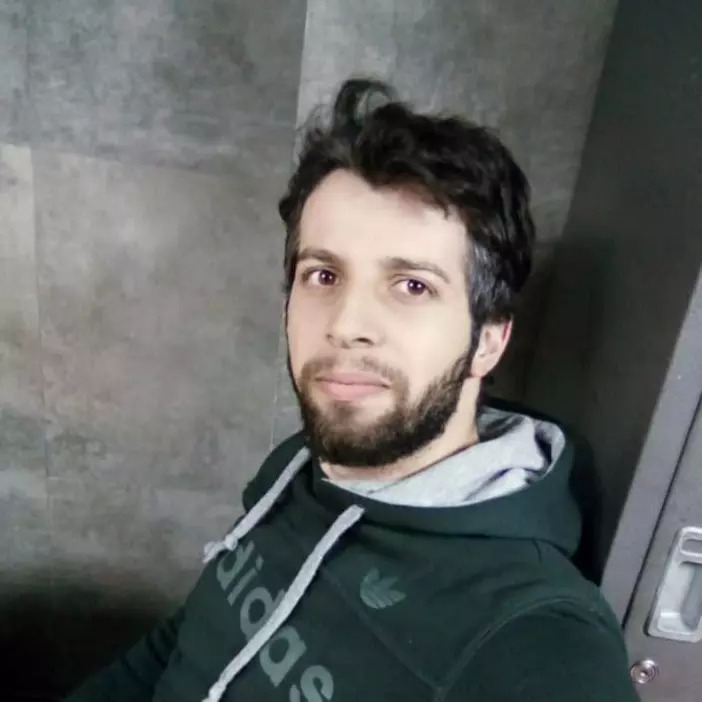
\includegraphics[width=1\textwidth, trim={0 0.6cm 0cm 0}, clip]{me.jpg} % Picture
	\end{minipage} \hfill
\end{tcolorbox}

%%% Sections %%%
\begin{minipage}{0.7125\textwidth} % Main Panel (e.g. Education, Work Experience)
	\begin{tcolorbox}[height=0.8\textheight, grow to left by=0.55cm,colframe=white,colback=white]

		%%%%%%%%%%%% Education %%%%%%%%%%%%
		\mySection{Education}
		\entryFocusDesc{10.2021 - current}
		{PhD of Applied Mathematics}{at Tarbiat Modares}
		{Numerical Analysis}
		{ \begin{compactitem}[-]
				\item Average: 18.49
			\end{compactitem}
		}

		\entryFocusDesc{10.2018 - 07.2021}
		{Master of Applied Mathematics}{at Tarbiat Modares}{Numerical Analysis}
		{\begin{compactitem}[-]
				\item Average: 16.08
				\item Thesis:
				Application of Machine Learning Algorithms in Modelling and Solving Parabolic Partial Differential Equations
			\end{compactitem}
		}

		\entryDesc{10.2013 - 07.2018}
		{Bachelor of Mathematics}{at Urmia Nazloo}
		{\begin{compactitem}[-]
				\item Average: 12.54
			\end{compactitem}
		}




		%%%%%%%%%%%% Work experience %%%%%%%%%%%%
		\mySection{Work experience}

		\entryFocusDesc{10.2023 - 03.2024}
		{Teacher Assistant}{at Numerical Learning Methods}
		{Python based learning problem solving}
		{\begin{compactitem}[-]
				\item Providing Lectures of Python Programming
				\item Solving Problems of TextBook using Python
				\item Providing Visual Lectures of Python Simulations
			\end{compactitem}
		}

		\entryFocusDesc{10.2022 - 03.2023}
		{Teacher Assistant}{at Digital Image Processing}
		{Python based Digital Image Processing}
		{\begin{compactitem}[-]
				\item Providing Lectures of Python Programming
				\item Solving Problems of TextBook using Python
				\item Providing Visual Lectures of Python Simulations
			\end{compactitem}
		}

		\entryFocusDesc{10.2021 - 03.2022}
		{Teacher Assistant}{at Machine Learning Basics}
		{R Programming and utils for Machine Learning}
		{\begin{compactitem}[-]
				\item Providing Lectures of R Programming
				\item Solving Problems of TextBook using R
			\end{compactitem}
		}

		%%%%%%%%%%%% Publications %%%%%%%%%%%%
		\mySection{Publications}
		\entryFocus{01.2023}
		{An efficient meshless method to approximate semi-linear stochastic evolution equations}
		{Mahdi Jalili, Rezvan Salehi, Mehdi Dehghan}

		\entryFocus{12.2021}
		{The approximate solution of one dimensional stochastic evolution equations by meshless methods}
		{Mahdi Jalili, Rezvan Salehi}

		%%%%%%%%%%%% Interests %%%%%%%%%%%%
		\mySection{Interests}
		\entryNoDate{Mathematics and Applications, Linux, Python, C++, MATLAB, \LaTeX}

	\end{tcolorbox}
\end{minipage}
\begin{minipage}{0.23\textwidth} % Side Panel (e.g. Skills, Links, Languages, etc.)
	\begin{tcolorbox}[height=0.8\textheight, grow to right by=0.5cm, colback=accent,colframe=accent,arc=1mm]
		% Skills, the skill level is drawn as bars, input: skill name and an array starting from 0 and ending before 4
		\vspace{0.5em}
		\subsection*{Programming Skills}
		\skill{Python}{5}
		\skill{LaTeX}{4}
		\skill{MATLAB}{4}
		\skill{R}{3}
		\skill{C++}{3}

		\vspace{2em}
		\subsection*{Languages}
		\skill{Turkish (Native)}{5}
		\skill{English (B2 Proficiency)}{4}
		\skill{Persian (Second Native)}{4}


		\vspace{2em}
		\subsection*{Additional}
		\skill{Linux (LPIC 2)}{5}
		\skill{Git}{4}
		\skill{SSH}{3}
	\end{tcolorbox}
\end{minipage}

\end{document}
